\chapter{Introduction}

% Apply a background image to the epigraph region
\begin{tikzpicture}[remember picture, overlay]
  % Place the image (background) in the epigraph area
  \node[anchor=north west, opacity=0.5, scale=1.4,yshift=0.2cm,xshift=-0.2cm] at (current page.north west) {
    \includegraphics[width=\paperwidth]{../plots/0_images/hubble_ultra_deep.png} % Your image path
  };
\end{tikzpicture}



\epigraph{Who really knows? \\ Who will unfold it? \\ How did this Universe formed?\\ Where does it come from? \\ Gods came after the creation. \\ Then, who really witnessed the origin of this existence?} {Rigved X.129.6}



\section{Prespective on the Subject}
\textit{Have you ever wondered why the Sun shines, why stars exhibit different colors, or what the structure of the Milky Way is? How far is the Andromeda galaxy from Earth? Do structures larger than galaxies exist? How far into the Universe can we observe? And perhaps most intriguingly, are we alone in this vast cosmos?}

\subsection{Astrophysics, Astronomy and Cosmology}
Such fundamental questions have been explored—though not yet fully answered—through the field of astrophysics. By observing the Universe across vast distances and in all directions using various wavelengths and observational techniques, scientists have begun to unravel these cosmic mysteries. Astrophysics is inherently interdisciplinary, drawing upon principles from physics, chemistry, geology, computer science, and other fields to construct a coherent understanding of the Universe and our place within it. Astrophysicists investigate the interactions and evolution of celestial bodies, the dynamics of cosmic ecosystems, and the potential existence of extraterrestrial life.

Astronomy can be regarded as the precursor to astrophysics, focusing on the study of the positions, motions, brightness, and classifications of celestial objects. This observational approach is essential for modeling the dynamics of the Universe, allowing us to predict astronomical events such as solar and lunar eclipses, planetary conjunctions, stellar motion within the Galaxy, and to map the observable Universe. In essence, astronomy addresses "what" and "where" questions, while astrophysics delves into "how" and "why" inquiries. 

On a broader scale, cosmology treats the Universe as a unified system. It explores the shape, age, evolution, and ultimate fate of the Universe. In examining the vast spectrum of spatial scales, galaxies appear as the fundamental units, organized into larger structures such as galaxy clusters and superclusters, all interconnected by cosmic filaments of gas and dark matter. These large-scale structures collectively form the cosmic web.

Constrained by observational data, cosmology is closely aligned with philosophical inquiry and stands as one of the oldest scientific fields studied by humanity.

\subsection{Spectrum of Spatial Scale}
The hymns of Rigved, originally composed in Sanskrit over 2,500 years ago, remain strikingly relevant to modern cosmology. They reflect a deep philosophical inquiry into the origins, scales and structure of the Universe—an inquiry that continues today as our understanding evolves through ongoing observation and theoretical advancement. In this section, I provide a brief overview of the Universe's structure as revealed by contemporary astronomical observations.

\begin{figure}[ht!]
\begin{center}
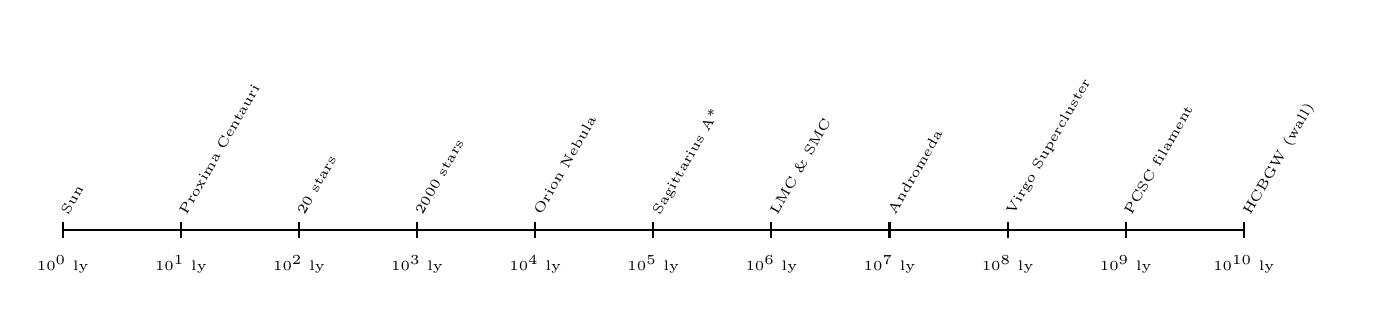
\begin{tikzpicture}
    % Parameters
    \def\n{10}
    \def\length{15}
    \def\spacing{\length/\n}

    % Labels array
    \def\labels{{"Sun", "Proxima Centauri", "20 stars", "2000 stars", "Orion Nebula", "Sagittarius A*", 
                 "LMC \& SMC", "Andromeda", "Virgo Supercluster", 
                 "PCSC filament", "HCBGW (wall)"}}

    % Draw base line
    \draw[thick] (0,0) -- (\length,0);

    % Draw tick marks, numbers and rotated labels
    \foreach \i in {0,...,10} {
        \pgfmathsetmacro{\x}{\i*\spacing}
        \draw[thick] (\x,0.1) -- (\x,-0.1); % Tick
        \node[below, font=\tiny] at (\x, -0.2) {$10^{\i}$ ly};      % Number
        
        % Multi-line labels with a 2-line approach for long labels
        \node[above, font=\tiny, text width=2.5cm, rotate=60, anchor=north west] at (\x-0.2,+0.2) 
            {\pgfmathparse{\labels[\i]}\pgfmathresult}; % Label
    }
\end{tikzpicture}
\caption{Cosmic distances span from nearby stars to the largest known structures in the universe, measured on scales of light-years, typically up to the order of 10. Each label represents either the distance to a notable astronomical object or the size of a vast cosmic region. The diameter of the observable universe is roughly 93 billion light-years, which is nearly the order of 11.}
\end{center}
\end{figure}



\subsubsection*{Milky Way in Presepective}
 
To gain perspective on the size of the Universe, it is useful to compare distances across different scales. For instance, the nearest star to the Sun is Proxima Centauri, located approximately 4.24 light-years away.  By definition, one light-year is the distance that light travels in a vacuum over the course of one year, equivalent to approximately 9.46 trillion kilometers. Within a 10 light-year radius of the Sun, there are about 20 stars, and nearly 2,000 stars lie within 100 light-years. The stars of the Orion Belt are situated at distances ranging from 800 to 1,300 light-years.

The Milky Way Galaxy is characterized by three major spiral arms—Perseus, Scutum-Centaurus, and Sagittarius—and three minor arms: the Orion Spur, Carina-Sagittarius, and Norma Arms. Our Solar System is located within the Orion Spur, a region containing millions of stars, situated between the Perseus Arm on the inner side and the Scutum-Centaurus Arm on the outer side.

\begin{figure}[htbp]
  \centering
  % Subplot 1
  \begin{subfigure}[b]{0.35\textwidth}
    \includegraphics[width=\textwidth]{../plots/0_images/Nearby_Stars.png}
  \end{subfigure}
  \hfill
  % Subplot 2
  \begin{subfigure}[b]{0.64\textwidth}
    \includegraphics[width=\textwidth]{../plots/0_images/milky_way.png}
  \end{subfigure}

  \caption{\textit{Left:} Stars located within 15ly. \textit{Right:} A segment of the Milky Way depicting the Solar System and its neighboring nebulae located in the Orion–Cygnus Arm. The Galactic Center and other minor arms - Norma and Carina–Sagittarius - are also highlighted.}
  \label{solar_system}
\end{figure}




The Perseus and Scutum-Centaurus arms seem to converge near the ends of the Long Bar, a stellar structure that stretches roughly 15,000 light-years and extends through the Galactic center. At the galaxy's core lies Sagittarius A*, a supermassive black hole believed to be the rotating nucleus of the galaxy. It is located approximately 27,000 light-years from Earth. Collectively, these elements contribute to the Milky Way's characteristic spiral disk structure, with a prominent bulge at its center.

\subsubsection*{Galactic Halo and Galaxies around}
The Milky Way’s spiral structure spans roughly 100,000 light-years in diameter, and is surrounded by a spherical halo extending up to three times that size. This halo hosts numerous satellite galaxies. One of the most prominent and easily visible from the southern hemisphere is the Large Magellanic Cloud (LMC), the Milky Way’s largest satellite galaxy, located about 160,000 light-years (50 kpc) away. The LMC itself has a satellite—the Small Magellanic Cloud (SMC)—located approximately 200,000 light-years (60 kpc) from Earth. In total, the Milky Way has over 50 known satellite galaxies. Its nearest large galactic neighbor is the Andromeda Galaxy (M31), situated around 2.54 million light-years (778 kpc) away. Andromeda is roughly two to three times larger than the Milky Way.


\begin{figure}[htbp]
  \centering
  % Subplot 1
  \begin{subfigure}[b]{0.36\textwidth}
    \includegraphics[trim= 0pt 0pt 0pt 45pt, clip, width=\textwidth]{../plots/0_images/Milky_Way_side_view.png}
  \end{subfigure}
  \hfill
  % Subplot 2
  \begin{subfigure}[b]{0.63\textwidth}
    \includegraphics[width=\textwidth]{../plots/0_images/local_group.png}
  \end{subfigure}

  \caption{\textit{Left:} Side view of the Milky Way, depicting its components and satellite galaxies, notably the Large and Small Magellanic Clouds (LMC and SMC). \textit{Right:} Spatial distribution of galaxies within the Local Group, dominated by the Milky Way and Andromeda galaxies. Source: Wikipedia - Pablo Carlos Budassi (left) and Andrew Z. Colvin (right)}
  \label{milkyway}
\end{figure}




Expanding the view to a radius of 10 million light-years, the region contains about 56 galaxies, among which the Milky Way and Andromeda are the most massive and gravitationally dominant. This collective of galaxies is known as the Local Group, which itself resides in the central region of the Virgo Supercluster.

\begin{figure}[htbp]
  \centering
  % Subplot 1
    \includegraphics[width=\textwidth]{../plots/0_images/local_superclusters.png}
  \caption{Galaxy supercluster and voids within $10^9$ ly of Virgo Supercluster. Source: Andrew Z. Colvin (Wikipedia)}
  \label{voids}
\end{figure}




\subsubsection*{Galaxy Clusters to Superclusters}
As we consider larger cosmic scales, the megaparsec (Mpc) becomes a more convenient unit for measuring distances. One megaparsec is approximately 3.26 million light-years. The Virgo Supercluster, which includes the Local Group, the Virgo Cluster, and several other galaxy clusters, spans a diameter of about 33 Mpc (roughly 100 million light-years).


The Virgo Supercluster is situated within the Laniakea Supercluster, a much larger structure that encompasses a volume about five times greater and contains approximately 100,000 galaxies. Other major regions within Laniakea include the Pavo-Indus Supercluster, the Southern Supercluster, and the Hydra-Centaurus Supercluster.

At the heart of Laniakea, within the Hydra-Centaurus Supercluster, lies a region of maximum gravitational attraction known as the Great Attractor. Most galaxies within Laniakea—including the Milky Way—are being gravitationally drawn toward this region.

\subsubsection*{Cosmic Web: Filaments, Walls and Voids}
The Laniakea Supercluster, along with the Shapley, Hercules, Coma, and Perseus–Pisces Superclusters, are all part of a vast galactic filament known as the Pisces–Cetus Supercluster Complex (PCSC). This structure is estimated to be approximately 1 billion light-years long and 150 million light-years wide, making it one of the largest known structures in the observable Universe.

Adjacent to it lies an even slightly larger filament known as the Perseus–Pegasus Filament. However, the largest known galaxy filament is the Hercules–Corona Borealis Great Wall (HCBGW), which stretches up to 10 billion light-years in length—roughly one-tenth the diameter of the observable Universe. Billions of such galaxy filaments, interwoven with gigantic cosmic voids, form the cosmic web—a vast, interconnected structure that defines the large-scale architecture of the Universe. This grand-scale pattern of matter distribution is illustrated in Figure \ref{scal}.  


\begin{figure}[htbp]
	\includegraphics[width=\textwidth]{../plots/0_images/scales}
	\caption{Large-scale structure of the Universe illustrating the cosmic web. \textit{Source: S. Stapelberg, Structures blog from the University of Heidelberg}}\label{large_scale}
\end{figure}





\section{Historical Background and Development}
Advancements in observational technology have enabled the exploration of the Universe at unprecedented depths and resolutions. These technological developments have profoundly influenced our understanding, offering novel perspectives on the evolutionary history and large-scale structure of the cosmos. This section presents a concise overview of the historical progression of astronomical research, with particular emphasis on pivotal discoveries and theoretical developments made over the past century that have fundamentally shaped contemporary cosmology.

\subsection{Distance Determination beyond the Galaxy, 1920s}
Prior to the twentieth century, the Milky Way (MW) was widely regarded as the entirety of the Universe, believed to be approximately 1.8 billion years old. The Sun was thought to occupy the central position in the cosmos, while other galaxies were misidentified as localized gaseous clouds within the Milky Way, and were classified as \textit{spiral nebulae}. This fundamental misunderstanding regarding the scale of the Universe led to a protracted debate among astronomers, most notably the Shapley–Curtis Debate in 1920, between Harlow Shapley and Heber Curtis.

A key issue underlying this debate was the inability to accurately determine the distances to these spiral nebulae. The breakthrough came with the discovery of the period–luminosity relation for pulsating stars—specifically, Cepheid variables—by Henrietta Swan Leavitt in 1912 \citep{1908leavitt,1912leavitt}. Her empirical relation, expressed as $m_{max} \propto log P$, enabled astronomers to estimate extragalactic distances with far greater accuracy. This development proved instrumental in resolving the scale of the Universe and is illustrated in Figure \ref{Leavitt-Hubble}.

\begin{figure}[ht!]
	\centering
	\begin{subfigure}[t]{0.45\textwidth}
         \centering
         \includegraphics[width=0.75\textwidth]{../plots/0_images/1912_Leavitt}
	 \label{Leavitt}
     \end{subfigure}
	\hfill
     \begin{subfigure}[t]{0.49\textwidth}
         \centering
         \includegraphics[width=\textwidth]{../plots/0_images/1929_Hubble}
	     \label{Hubble}
     \end{subfigure}
	\caption{Two remarkable discoveries of early twentieth century: a) Leavitt Law: Period (in logarithmic scale) of 25 Cepheids (of Small Magellanic Cloud) correlated with their maximum and minimum brightness. \cite{1912leavitt} b) Hubble Law: Increasing recession velocity of galaxies with respect to distance suggesting an expanding Universe. \cite{1929hubble}}\label{Leavitt_Hubble}
\end{figure}




\begin{notebox}[sharp corners, width=\textwidth]{Knowledge of Distance is fundamental in astronomy.}
Distance enables us to convert the sky’s seemingly two-dimensional projection into a three-dimensional representation of the Universe. Once the distance to a bright object is known, its true luminosity can be determined, allowing us to infer its size, mass, age and other physical characteristics.
\end{notebox}




\subsection{Expansion of the Universe}
In 1923, using the most advanced instrument of his time, the 100 - inch (2.5 m) Hooker Telescope, Edwin Hubble observed the Andromeda \textit{spiral nebula} (M31) and successfully resolved a Cepheid variable star within it. By applying the Leavitt Law (period–luminosity relation) \citep{1925hubble}, he estimated the distance to M31 and demonstrated that it lay far outside the boundaries of the Milky Way. This discovery effectively resolved the "Great Debate" in favor of Heber Curtis, confirming that Andromeda is a separate galaxy, and that the Milky Way is just one of billions of galaxies in the Universe.

Continuing his observations of Cepheid variables, Hubble measured distances to additional galaxies and identified a key relationship: the recessional velocity of a galaxy increases with its distance from the observer, expressed as $v \propto D$ \citep{1929hubble}; see Figure \ref{Leavitt-Hubble}. This empirical relation, now known as Hubble’s Law, led to the revolutionary conclusion that the Universe is expanding in all directions - a concept that contradicted Einstein’s earlier static model of the Universe \citep{1917einstein}. The constant of proportionality in this relation, known as the Hubble constant $H_0$, is of great cosmological importance, as it provides a measure of the expansion rate and thus the age of the Universe.

\subsection{The Big Bang Model, 1930s}
In the meantime, building upon Einstein’s theory of general relativity, Georges Lemaître independently arrived at the conclusion of an expanding Universe, and proposed that its earliest state was an immensely hot and dense origin \citep{1931lemaitre}. Further theoretical advances were made in 1948, when Alpher and Herman \citep{1948alpher} refined Gamow’s model of the early Universe \citep{1948gamow} and predicted the existence of cosmic microwave background (CMB) radiation—a thermal remnant of the Big Bang - at a temperature of approximately 5K.

This prediction was confirmed in 1965, when Arno Penzias and Robert Wilson detected microwave radiation with a temperature of 3.4 $\pm$ 1K using the Holmdel Horn antenna \citep{1965penzias}. Their discovery provided strong empirical support for the Big Bang model, which today stands as the standard cosmological model, describing the origin, evolution, and large-scale structure of the Universe.

\subsection{Composition of Stars}
Parallel advancements in quantum physics during the early twentieth century significantly enhanced our understanding of stellar evolution. In 1917, Arthur Eddington proposed a thermodynamic model based on free radial oscillations to explain the pulsations observed in Cepheid variable stars \citep{1917eddington}. Building on this framework, he hypothesized in 1920 that the primary source of stellar energy is hydrogen fusion into helium \citep{1920eddington}—a revolutionary idea at the time.

Further insights emerged from the study of stellar spectra. In her 1925 Ph.D. dissertation, Cecilia Payne (later Payne-Gaposchkin) demonstrated that hydrogen and helium are the most abundant elements in stars, contradicting the prevailing view that stars had compositions similar to Earth \citep{1925payne}. Her groundbreaking work established these two elements as the principal constituents of stellar matter. A comprehensive theoretical account of nuclear fusion reactions within stars was later formulated by Hans Bethe in 1939 \citep{1939bethe}, laying the foundation for modern stellar nucleosynthesis theory. It was a major leap in astronomy, as the physics of internal mechanics of stars was not well known priory, including the right mechanism behind the cyclic pulsation of Cepheid variable. 

\subsection{Age of the Universe, 1950s}
Studying stellar pulsations, Walter Baade discovered that Cepheid variables are divided into two distinct populations: Type I (classical Cepheids), which are brighter, and Type II (W Virginis stars). His recalibration of the Cepheid distance scale led to a doubling of the estimated distance to the Andromeda Galaxy and a corresponding revision of the Universe’s age from 1.8 billion to 3.6 billion years \citep{1958baade}. This estimate was further refined by his student, Allan Sandage, who extended Leavitt’s relation into a period–color–luminosity law and revised the Hubble constant to 75 km/s/Mpc in 1958 \citep{1958sandage}, resulting in an updated estimate of the age of the Universe at approximately 14 billion years. Allan's estimation lies near to modern value of Hubble constant.


\subsection{Technological Development, 1960s}
Despite numerous unresolved questions and theoretical challenges, technological advancements have significantly propelled research in astronomy, leading to major breakthroughs and providing deeper insights into the nature and evolution of the Universe. Beginning in the 1960s, the introduction of digital imaging in photometry revolutionized observational astronomy. The replacement of photographic plates with charge-coupled device (CCD) cameras markedly improved the accuracy, sensitivity, and precision of photometric measurements.

The deployment of space-based telescopes enabled observations across the entire electromagnetic spectrum, overcoming the limitations imposed by Earth’s atmosphere on ground-based instruments. Additionally, the detection of cosmic rays, neutrinos, and gravitational waves opened new avenues for studying celestial phenomena through multiple independent messengers, thereby giving rise to the field of \textit{multimessenger astronomy}. Concurrently, advances in high-energy particle physics uncovered the quantum-scale substructure of matter, contributing to more refined and physically grounded models of astrophysical processes. Collectively, these technological and theoretical developments have brought a paradigm shift in our understanding of the cosmos, marking the onset of what is often referred to as the golden era of modern astronomy.

\subsection{Composition of Universe}
Given the vastness of the universe, it is natural to wonder what it is made of. A simplified answer might be that it consists of energy and spacetime. However, energy manifests in several distinct forms undergoing different physical processes and laws. It can be heat, mass, radiation or of any other form. 

\begin{wrapfigure}{r}{0.45\textwidth}
	\begin{center}
		%\vspace{-1cm}
		\includegraphics[width=7cm]{../plots/0_images/uni_compo}
		\vspace{-1mm}
		\caption{The fractional composition of the Universe consists of dark energy (68 \%), dark matter (27 \%), and baryonic matter (5 \%) is depicted, with the contributions from radiation and other relativistic particles neglected.}
		\label{uni_composition}
		\vspace{-1cm}
	\end{center}
\end{wrapfigure}


In cosmological terms, ordinary matter, referred to as \textit{baryonic matter}, comprises electrons, protons, and neutrons, and constitutes only about 5\% of the total energy content of the universe. This baryonic matter forms the stars, galaxies, and large-scale structures we observe today. In addition to baryonic matter, dark matter represents another critical component of the cosmos. Dark matter is hypothesized to possess fundamentally distinct properties from ordinary matter, as it neither emits nor absorbs electromagnetic radiation, rendering it invisible. Its presence is inferred solely through its gravitational effects. Dark matter accounts for approximately 27\% of the universe's total energy content. Strong observational evidence for dark matter emerges from phenomena such as gravitational lensing, the anomalous rotation curves of galaxies, and the fine-scale anisotropies in the Cosmic Microwave Background (CMB). These observations, however, rely heavily on accurate distance measurements. For instance, the interpretation of gravitational lensing patterns and galaxy rotation curves depends critically on the precise determination of the distances to the lensed or orbiting objects. Despite its discernible gravitational influence, the precise nature and composition of dark matter remain unresolved, rendering it one of the most significant unsolved problems in contemporary astrophysics.

On cosmological scales, observational data further indicates that the universe is expanding at an accelerating rate, a phenomenon attributed to a hypothetical form of energy known as dark energy. Like dark matter, the exact nature of dark energy is still unknown, but it is postulated to comprise approximately 68\% of the total energy density of the universe. In stark contrast, other components, such as radiation, neutrinos, and various exotic non-baryonic particles, collectively account for less than 1\%. The study of the distribution and evolution of these components remains a vibrant and evolving field of inquiry in modern cosmology.

The determination of the relative proportions of these matter and energy components hinges on precise distance measurements across cosmic scales, as these distances are pivotal in estimating both the observed brightness and redshift of distant objects—crucial factors in reconstructing the universe’s overall composition.


\subsubsection{$\Lambda$CDM Cosmological Model}

By integrating observational data with the initial conditions established by Big Bang cosmology, scientists have formulated a standard cosmological model known as the $\Lambda$CDM (Lambda Cold Dark Matter) model. This model is defined by key parameters, including the densities of dark energy, dark matter, and baryonic matter; the Hubble constant ($H_0$); the scalar spectral index (which describes primordial density fluctuations); and the curvature parameter (which determines the geometry of the universe). Many of these parameters are tightly constrained using cosmic microwave background (CMB) measurements and are supported by various independent astronomical observations.

Accurate knowledge of cosmic distances is essential for estimating these parameters. The expansion rate, for instance, is inferred from the relationship between redshift and distance (the Hubble Law), while the discovery of the universe's acceleration was made possible by analyzing the luminosity of distant Type Ia supernovae.

Despite their differences in physical nature, the topics above share a common goal: the determination of distances to astronomical objects in order to accurately derive other physical parameters, such as size, mass, and age. Building on this idea, the primary focus of my master’s thesis is to explore distance determination methodologies, with a particular emphasis on the Leavitt Law, and to improve its accuracy by identifying and addressing sources of systematic errors. With final remarks on results implication, the last chapter concludes this thesis. 

The color gradient angular map of the sky shown in the introduction page is a snapshot of the early Universe, captured by the Planck satellite, a mission commissioned by the European Space Agency (ESA) and operational from 2009 to 2013. This map represents the Cosmic Microwave Background (CMB) radiation, which is the faint afterglow of the Big Bang. The temperature fluctuations across the sky observed in the CMB are the remnants of small density variations in the very early Universe. Over billions of years, these minute fluctuations grew due to gravitational attraction, eventually forming the large-scale structures of the Universe, including galaxies and galaxy clusters that we observe today.

The CMB is the most ancient relic we can witness from the early Universe, offering a direct glimpse into the conditions that prevailed just 380,000 years after the Big Bang. These observations allow scientists to infer important properties of the Universe's early state, such as its age, composition, and rate of expansion. One of the most significant results derived from the Planck data is the precise determination of the Hubble constant ($H_0$), which quantifies the current rate of expansion of the Universe. The value of $H_0$ is crucial for understanding the Universe's past and predicting its future evolution. 

When observing the Universe at great depths, we are essentially looking into the past, as light takes time to travel through space. This fundamental property allows us to study the early Universe and its evolution. One method of measuring the expansion rate of the Universe involves determining the distance to the farthest observable objects—essentially, measuring the distance to the cosmological horizon, the farthest point from which light has had time to reach us since the Big Bang.

To validate the Hubble constant ($H_0$) obtained from local measurements, we use a method known as the cosmic distance ladder. This method involves calibrating several different distance measurement techniques, each suitable for different scales of the Universe. These methods begin with relatively nearby objects and work outward to increasingly distant galaxies, eventually reaching the cosmological scale, where measurements can be compared to the results obtained from the Planck mission and other independent methods. By calibrating each step of the distance ladder, we can achieve a more accurate and consistent measure of cosmic distances, which in turn helps refine our understanding of the expansion rate of the Universe.

However, recent studies have revealed a discrepancy in the measured values of the Hubble constant, especially when comparing results from local measurements (such as Cepheid variable stars and the Tip of the Red Giant Branch method) to those obtained from the cosmic microwave background (CMB) observations, like those from the Planck mission. This discrepancy has come to be known as the $5-\sigma$ Hubble Tension. It refers to a statistical difference at the 5-sigma level, indicating a significant mismatch between the two methods. This tension has sparked a great deal of debate in the cosmological community, leading to numerous investigations into potential new physics that might explain the difference.


\subsection{Cosmic Distance Ladder and Hubble Constant}

One of the most pressing issues in modern cosmology is the growing discrepancy in the measured value of the Hubble constant ($H_0$)—the rate of expansion of the universe. Early-universe measurements, primarily derived from observations of the Cosmic Microwave Background (CMB) using the Planck satellite and interpreted within the $\Lambda$CDM cosmological model, yield a value for $H_0$ that significantly differs from those obtained via direct measurements in the local universe \citep{2018planck, 2021freedman}. This tension, now known as the \textit{Hubble tension}, challenges our understanding of cosmology and may point to new physics or systematic errors yet to be uncovered.

Late-universe estimates of $H_0$ are derived by correlating redshifts with distances of astronomical objects. Because no single method spans the full range of cosmic distances, astronomers rely on a sequence of interconnected techniques known as the \textit{cosmic distance ladder}. Each “rung” of the ladder is calibrated by more fundamental, closer-range methods to extend reliable distance measurements farther into the universe.


\begin{wrapfigure}{r}{0.45\textwidth}
	\begin{center}
		\vspace{-1cm}
		\includegraphics[width=7cm]{../plots/0_images/ladder}
		\vspace{-1mm}
		\caption{An instance of Cosmic Distance Ladder calibrating Leavitt Law with parallax, SNIa with Leavitt Law and Hubble Law with SNIa based distances. \citep{2022riess}}
		\label{ladder}
		\vspace{-1cm}
	\end{center}
\end{wrapfigure}




A key breakthrough in refining the distance ladder came from Adam Riess and collaborators, who studied Type Ia supernovae (SNIa) in distant galaxies. These explosive events, originating from white dwarf mergers, follow a predictable relation between their intrinsic brightness and the width of their light curves. By calibrating SNIa with Cepheid variable stars via the Leavitt Law, Riess extended high-precision distance measurements from the local 30 Mpc range ($\sim 10^8$ ly, Cepheid-based) to beyond 1000 Mpc ($ \sim 10^{10}$ ly) using SNIa as \textit{standard candles}—objects with known intrinsic luminosity \citep{1998riess}.

Figure~\ref{ladder} illustrates the cosmic distance ladder, starting from geometric parallax for nearby stars, advancing through Cepheid variables, and culminating in SNIa-based distances for high-redshift galaxies. Using this refined framework and fitting distances to the Hubble law derived:

\[
H_0 = 73.30 \pm 1.04 \; \text{km s}^{-1} \text{Mpc}^{-1}
\]
a result in $5\sigma$ tension with the Planck-inferred value under $\Lambda$CDM assumptions \citep{2022riess}. Resolving this discrepancy remains a top priority in cosmology, potentially revealing insights into dark energy, new particles, or modifications to the standard model of the universe.


\subsection{Golden Era of Astronomy - Gaia onwards}
The launch of the Gaia satellite by the European Space Agency (ESA) in 2013 marked a significant leap in modern astronomy. Utilizing the geometric parallax method with the baseline of Earth’s orbital diameter, Gaia has precisely measured the distances to over 1.8 billion stars within the Milky Way and its surrounding regions, while simultaneously conducting extensive photometric and astrometric observations of the sky. The exceptional accuracy of Gaia's measurements has established a new standard for distance calibration in astronomical research. This research work relies on distance measurements obtained from the parallax data of Gaia Data Release 3 (DR3). 

In 2021, the launch of the James Webb Space Telescope (JWST) by NASA further advanced the observational capabilities. With its sensitivity to the far-infrared spectrum, JWST has begun to reveal unprecedented details of the early Universe, including the formation of the first galaxies and stars. In addition to these missions, a number of major cosmological surveys and observatories—such as SDSS, Planck, and 2dFGRS—have already made transformative contributions to our understanding of the cosmos. Looking ahead, the commissioning of next-generation facilities, including the Vera C. Rubin Observatory, DESI, 4MOST, Euclid, SKA, and LISA, is expected to redefine the frontiers of observational astronomy and cosmology, setting new benchmarks for future research.


\section{Scope of this Thesis}


\begin{wrapfigure}{r}{0.4\textwidth}
	\begin{center}
		\vspace{-1.2cm}
		\includegraphics[width=6cm]{../plots/0_images/Storm2011.png}
		\vspace{0mm}
		\caption{\textit{K-band Period-Luminosity relation for Galactic Cepheid using IRSB distance.} Source: Storm J., 2011}\label{PLjesper}
		\vspace{-1cm}
	\end{center}
\end{wrapfigure}


The aim of this thesis is to improve the accuracy of Galactic Leavitt Law - a primary distance indicator of cosmic distance ladder. Note the large scatter in linear period-luminosity relation of Cepheids, giving uncertainity to the slope and zero point of the fit. Using such a period-luminosity relation as a reference for the next rung of distance scale leads to larger error in the measurements, making it crucial to have a tight PL relation in the first place - to gain a high confidence on the cosmological scale studies. To refine the Leavitt Law to its finest form, I will be taking following steps which will be briefly discussed in following chapters. 

\begin{itemize}
\item Identify and omit the outliers from BVIJHK photometric dataset of Galactic Cepheid.
\item Estimate intrinsic luminosity of observed targets using reddening and Gaia DR3 parallax. 
\item Determine error in distances and interstellar reddenings following the method of \cite{2017madore}.
\item Reformulate the Leavitt Law with distance-reddening corrected intrinsic luminosity of Cepheids.
\item Cross validate the calibrated Leavitt Law with Cluster Cepheid based Leavitt Law.
\item Apply the refined Leavitt Law on LMC and SMC Cepheids to determine their distances.
\end{itemize}

\subsection{Part I: Parameters of Leavitt Law}
The period-luminosity scatter plot requires primarily two parameters of Cepheid variables: a) accurate measurement of pulsation period, and b) accurate estimation of intrinsic luminosity of the respective Cepheid star. The Figure \ref{PLjesper} depicts an instance of Leavitt Law in K band, where distances to invidual stars measured by infrared surface brightness (IRSB) method \citep{2011storm}, and interstellar extinction derived using Fouque's extinction law \citep{2007fouque} and Fernie's reddening measurements \citep{1994fernie}. 

The pulsation periods of Cepheid variables are determined from light curves based on photometric observations spanning multiple pulsation cycles. This parameter is well-constrained for all Cepheid targets considered in this study. The primary focus of this research, however, lies in determining the second essential quantity—the intrinsic (absolute) luminosity of these stars. While telescopes measure the apparent luminosity, estimating the absolute luminosity requires correcting for both the distance the light has traveled and the attenuation caused by interstellar extinction.

Stellar light is subject to scattering and absorption as it traverses the interstellar medium, particularly through dust and gas clouds along the line of sight. Any imprecision in correcting for these effects leads to significant deviations from the expected linear relationship in the period-luminosity relation. Consequently, accurately quantifying the uncertainties in distance and interstellar reddening for each Cepheid is a central objective of this thesis.

The first part of this thesis is dedicated to a detailed examination of these parameters and their interdependencies, as outlined in the next chapters.

\subsection{Part II: Calibration Method and Dataset}
This part of thesis contains three chapters covering details on Galactic Cepheid dataset, calibration methodology, its related physics and comparision plots. The Galactic Cepheid dataset used in this thesis contains multiband photometric data in the BVIJHK bands. The extinction law developed by Cardelli et al. \citep{1989cardelli}, in combination with the total-to-selective extinction ratio adopted from Sandage \citep{2004sandage}, is employed to convert the color excess values compiled by Fernie into BVIJHK extinction. Using parallactic distance estimates from the Gaia mission and extinction, raw Leavitt Law are derived. 

The calibration technique used in this thesis is devised by Barry Madore \citep{2017madore}. Utilizing the reddening-free nature of the Wesenheit function \citep{1982madore}, the effect of reddening and distance errors on individual Cepheid can be decoupled and traced by comparing the residuals of BVIJHK period-luminosity relation with residual of period-wesehiet relation. In his paper, Madore had used V -  I based  wesenheit function to determine the errors and ultimately tighten the multiband PL relations. In this thesis, first, I applied the same method on B -  V, V -  K and J -  K based wesenheit functions, and compared the deviation in resulting distance-reddening error-pair for individual star, for each color index case. Secondly, I modified the methodology from generic wesenheit function to composite wesenheit function and repeated the exercise to derive the error-pairs for individual Cepheid for each color indicies. It lead to some crucial insights about wesenheit function and its dependency on the reddening ratio and color index. Finally, the calibrated Leavitt Law cross-validated with an additional dataset of 18 Galactic cluster Cepheids - more reliable distance measured by averaging parallax of the cluster members hosting the Cepheids. 

This part of the thesis ends with a discussion on the results. 

\subsection{Part III: Result Implications}

\subsubsection*{LMC \& SMC Distance}
To test the effectiveness, LMC and SMC distances have been derived for 24 versions of calibrated Leavitt Law, i.e. 6 photometric bands with 4 colors of wesenheit functions. With such multiple possibilities, a distance matrix can be made highlighting effectiveness of particular color index used in calibration, with respect to the rest.

In astronomy, distance is not just a measurement - it's the foundation upon which our understanding of the universe is built. From determining the true luminosity of celestial bodies to constraining the age, scale, and rate of expansion of the cosmos, accurate distance measurements are indispensable. The physical interpretation of almost every astronomical observation - be it the brightness of a star, the motion of a galaxy, or the composition of the universe - depends critically on knowing how far away the object lies. Throughout this section, we will see how the knowledge of distance informs our understanding of cosmic composition, the expansion rate, or the evolution of the Universe. 


